\section{Introduction}
% 1. Describe the Current Situtation
% Functions as a starting point and a common basis. Therefore it primarily contains recognizable and agreed points.
Advances in hardware that augment a user's physical actions have reignited dreams of overcoming human limitations, recovering lost abilities and simplifying skill acquisition~\citep{Goto2020-mw, Kunze2017-co}. However, augmented users often report dissociative experiences, frequently disrupting their sense of agency (SoA)~\citep{Gilbert2017-ze, Gilbert2019-uc}.

% 2. What is the complication, challenge identified
% Spells the reason for acting now. It contains threats / opportunities and the hurdles that need to be overcome.
Having a SoA means experiencing control of our own voluntary actions, instead of them feeling as randomly happening to us. It has frequently been shown that users are more likely to feel engaged and satisfied with an interaction, and are more likely to trust a system the more they experience SoA~\citep{Berberian2012-do, Miller2007-rb}. A key challenge to drive the adoption of human action augmentation then is to design for agency experience, so users feel as though they are in the ``driver's seat'' once again.

% 3. Question
% Asks the question how the hurdles of the Complication can be overcome. How can we prevent the threat or seize the opportunity? Also, what would be the benefits if the complication would be overcome?
% What have others done to address this and what do we propose "instead"
One goal of user augmentation is to increase reaction times, thereby making an interaction more efficient. Previous work on such augmentation scenarios has shown that an actuation preceding a movement by about 80 ms preserves agency~\cite{Kasahara2019-sk}. Evidence from cognitive neuroscience indicates that from around 200ms before a voluntary movement, users are unable to ``veto'' their self-initiated movement~\cite{Schultze-Kraft2016-bx}. Here, the \textit{key} aspect for SoA in action augmentation becomes apparent: External influences on the user's body need to be in line with the user's intention. 

In experimental settings, this is typically achieved by using strongly controlled `stimulus-response' paradigms. For example, reaction times when tapping on a touchscreen in response to a presented stimulus on screen, can be reduced by an augmentation device while maintaining SoA for the user~\cite{Kasahara2019-sk, Kasahara2021-gy}. In such controlled scenarios, the timing of the action augmentation can be tuned to be near optimal because the user behavior can be predicted with very high certainty to follow a previously presented stimulus. However, a key challenge remaining is to design systems that maintain agency during unpredictable actions of the user and \textit{without} control over the environment. In other words, how can we design a closed-loop system to deliver a \textit{natural} agency experience for users' augmented actions?

% [4. (short) Answer Teaser
% Provides the answer on how to overcome the hurdles. Explains how this will help deflect the threats or seize the opportunities.
% keep this very short]

\subsection{Preserving Agency using Brain Signals of the Intent to (Inter-) act}
% 4. (long) Anwser with teaser image
% Provides the answer on how to overcome the hurdles. Explains how this will help deflect the threats or seize the opportunities.
In this paper, we present a bleeding edge prototype to challenge the disruption in experiencing agency during action augmentation. We developed a brain-computer interface (BCI) that establishes a fast communication channel between a user's brain signals and a physical end effector. The AUGMENTATION system (from hereon referred to simply as \textit{system}) controls the user's muscles at the time of their \textit{intent to interact}, as measured through readiness potentials (RP) manifesting in the user's electroencephalogram (EEG)~\cite{Nguyen2023-me, Schurger2021-vp, Schultze-Kraft2016-bx, Schultze-Kraft2021-cu}. 

\begin{figure}[!h]
    \centering
    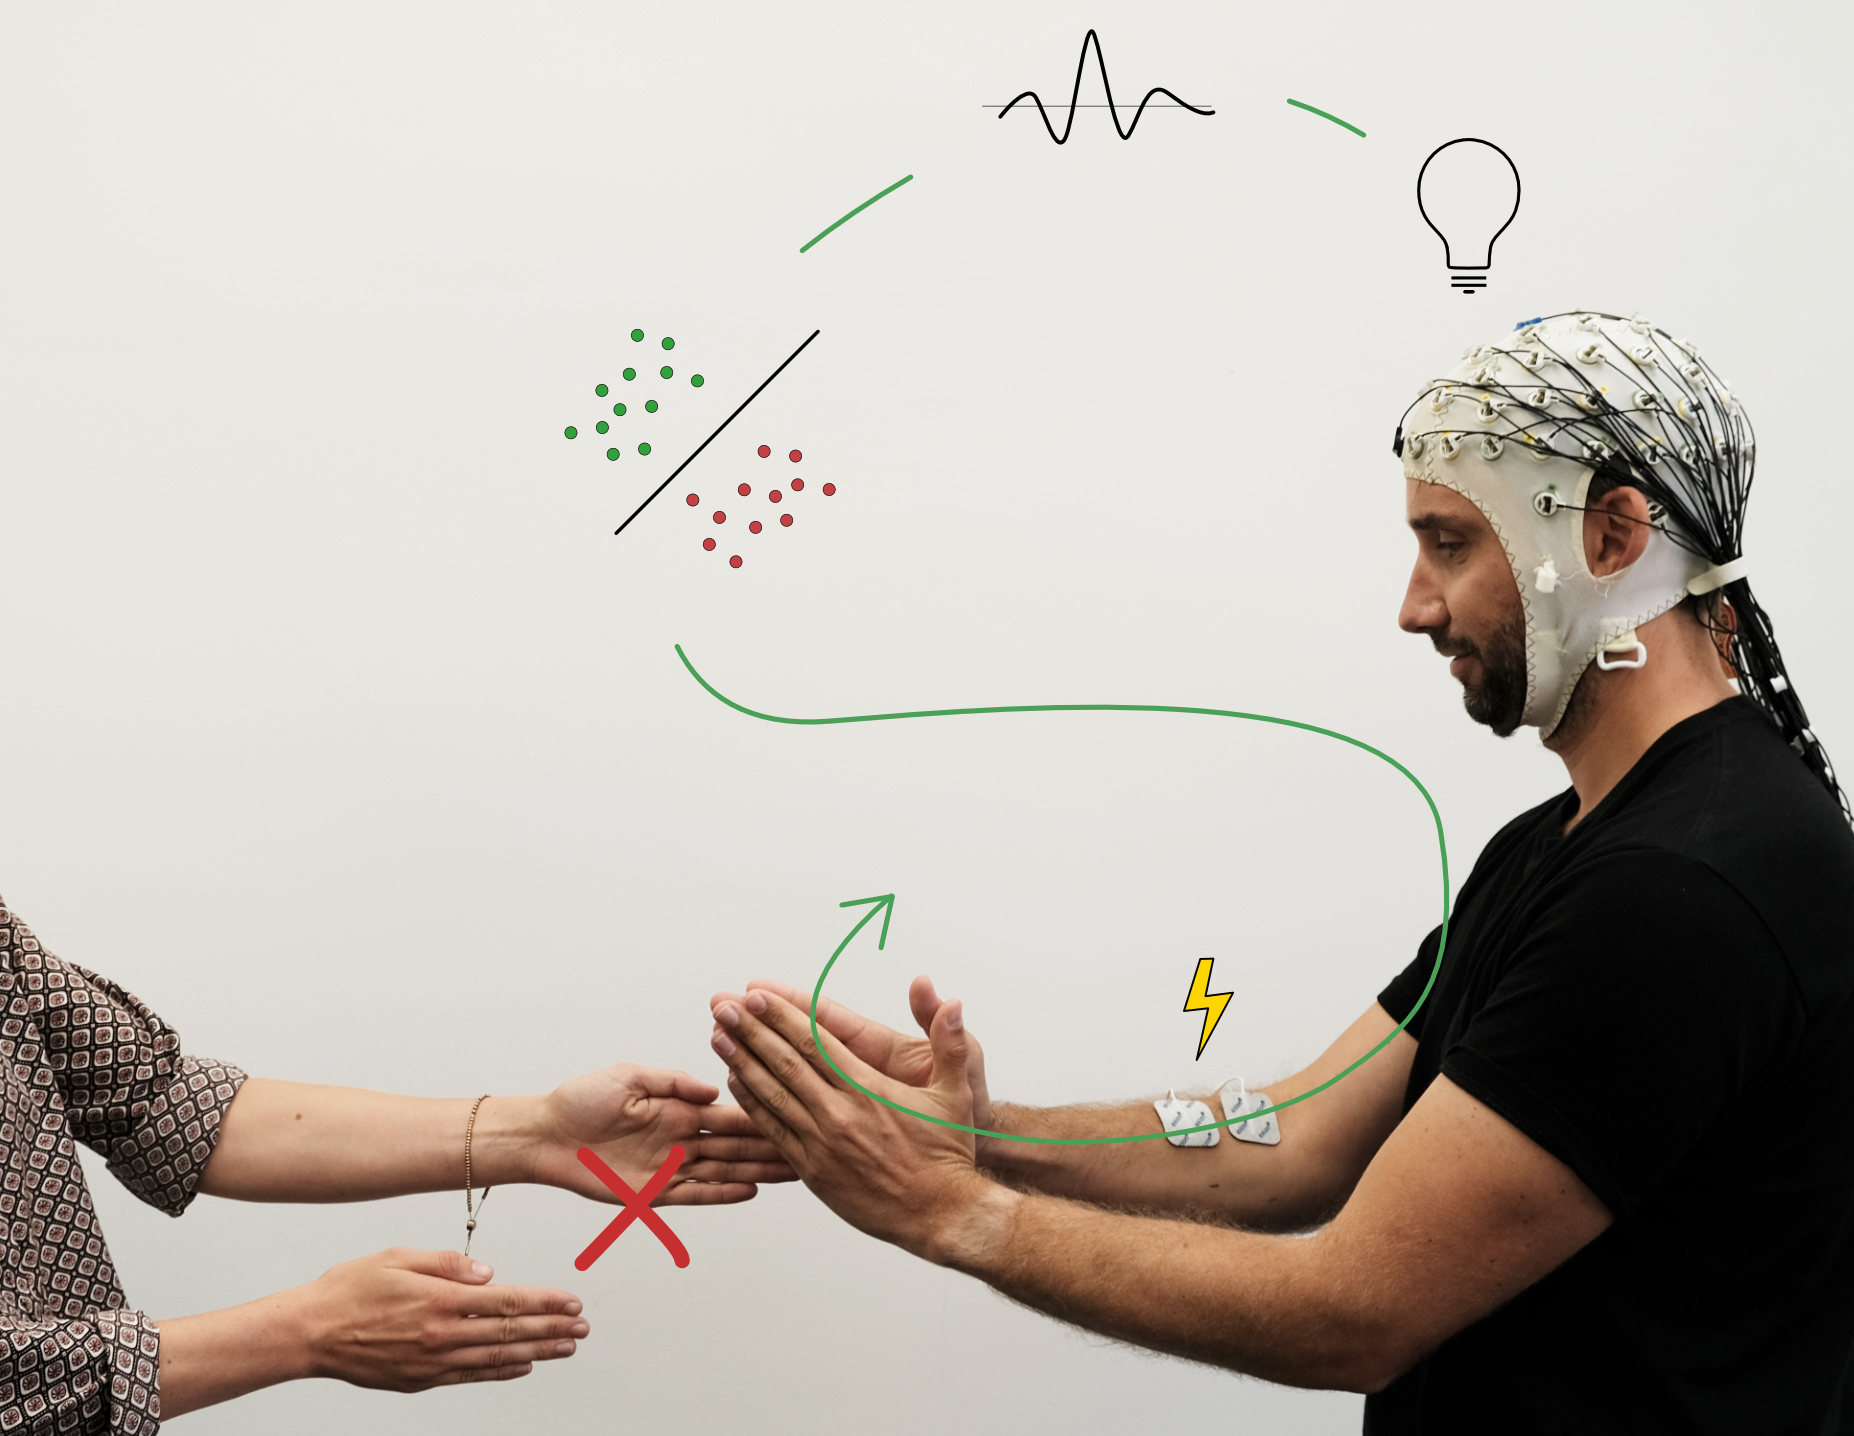
\includegraphics[width=\columnwidth]{figures/bci_game.png}
    \caption{Our Augmentation system: When participants feel the spontaneous urge to move, readiness potentials (RPs) are picked up in the user's EEG signals. A brain-computer interface (BCI) predicts the data to be in either of two classes: Idle or pre-movement. In the latter case, the user's hand is moved by trigger electrical muscle stimulation (EMS). Image presented with consent from participant.}
\end{figure}

% TODO merge this with the figure below
% \missingfigure{maybe small infographic here showing the connection from EEG volitional RP thought to EMS trigger on the Arm. <- better use this for the teaser image. Here better present the main results, i.e. SoA scores? -> Klaus comment: yes, but they don't have to be exclusive. The general setup with the LRP could appear with the main results both in the teaser or here? But the teaser would be more a visualization of the principle, no? That does not necessarily require real results but could show a hyperplane and data dots for examplification.}
% make this as an infographic with comic style drawing of augmented user and then the three pathways drawn
% \begin{figure}
%     \centering
%     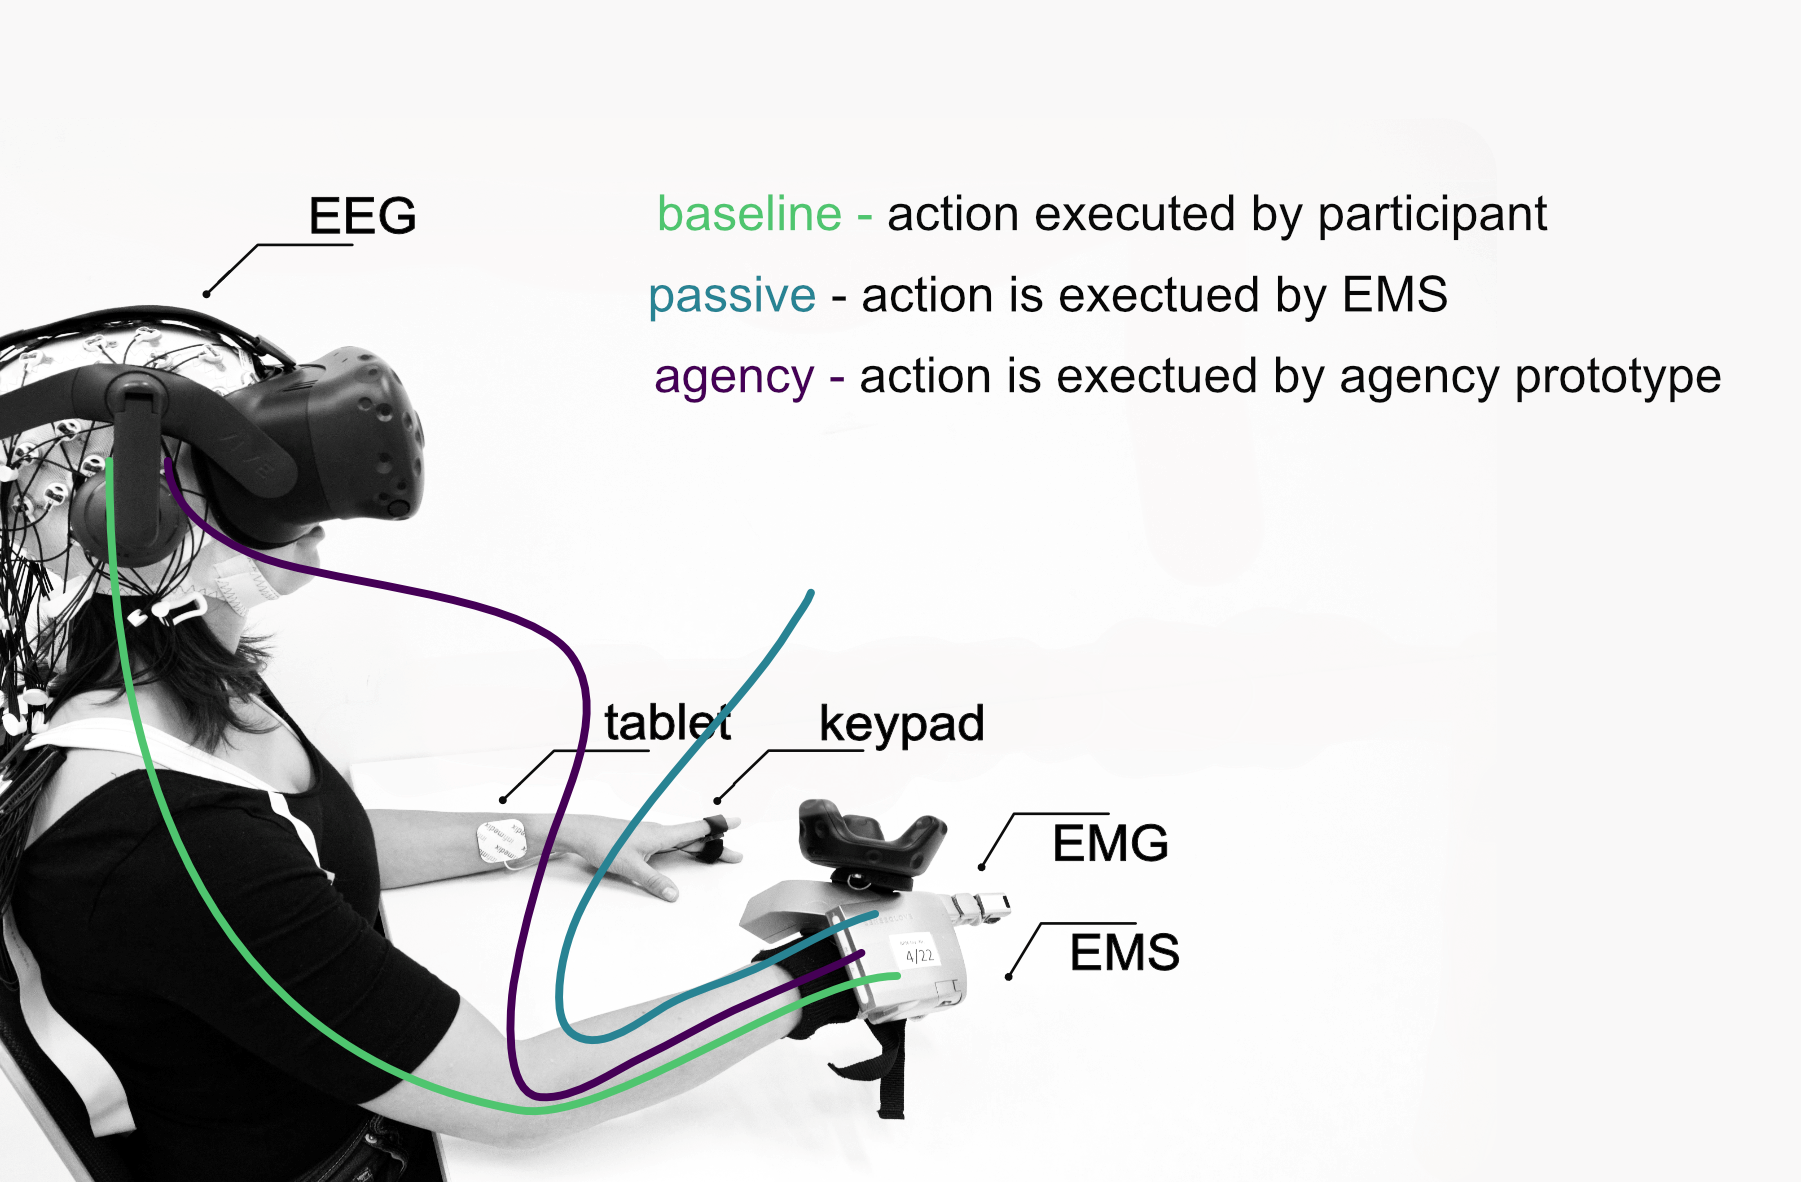
\includegraphics[width=\columnwidth]{figures/setup_conditions_draft_small.png}
%     \caption{draft apperatus and conditions}
%     \label{fig:setup}
% \end{figure}
% \begin{figure}[!h]
%     \centering
%     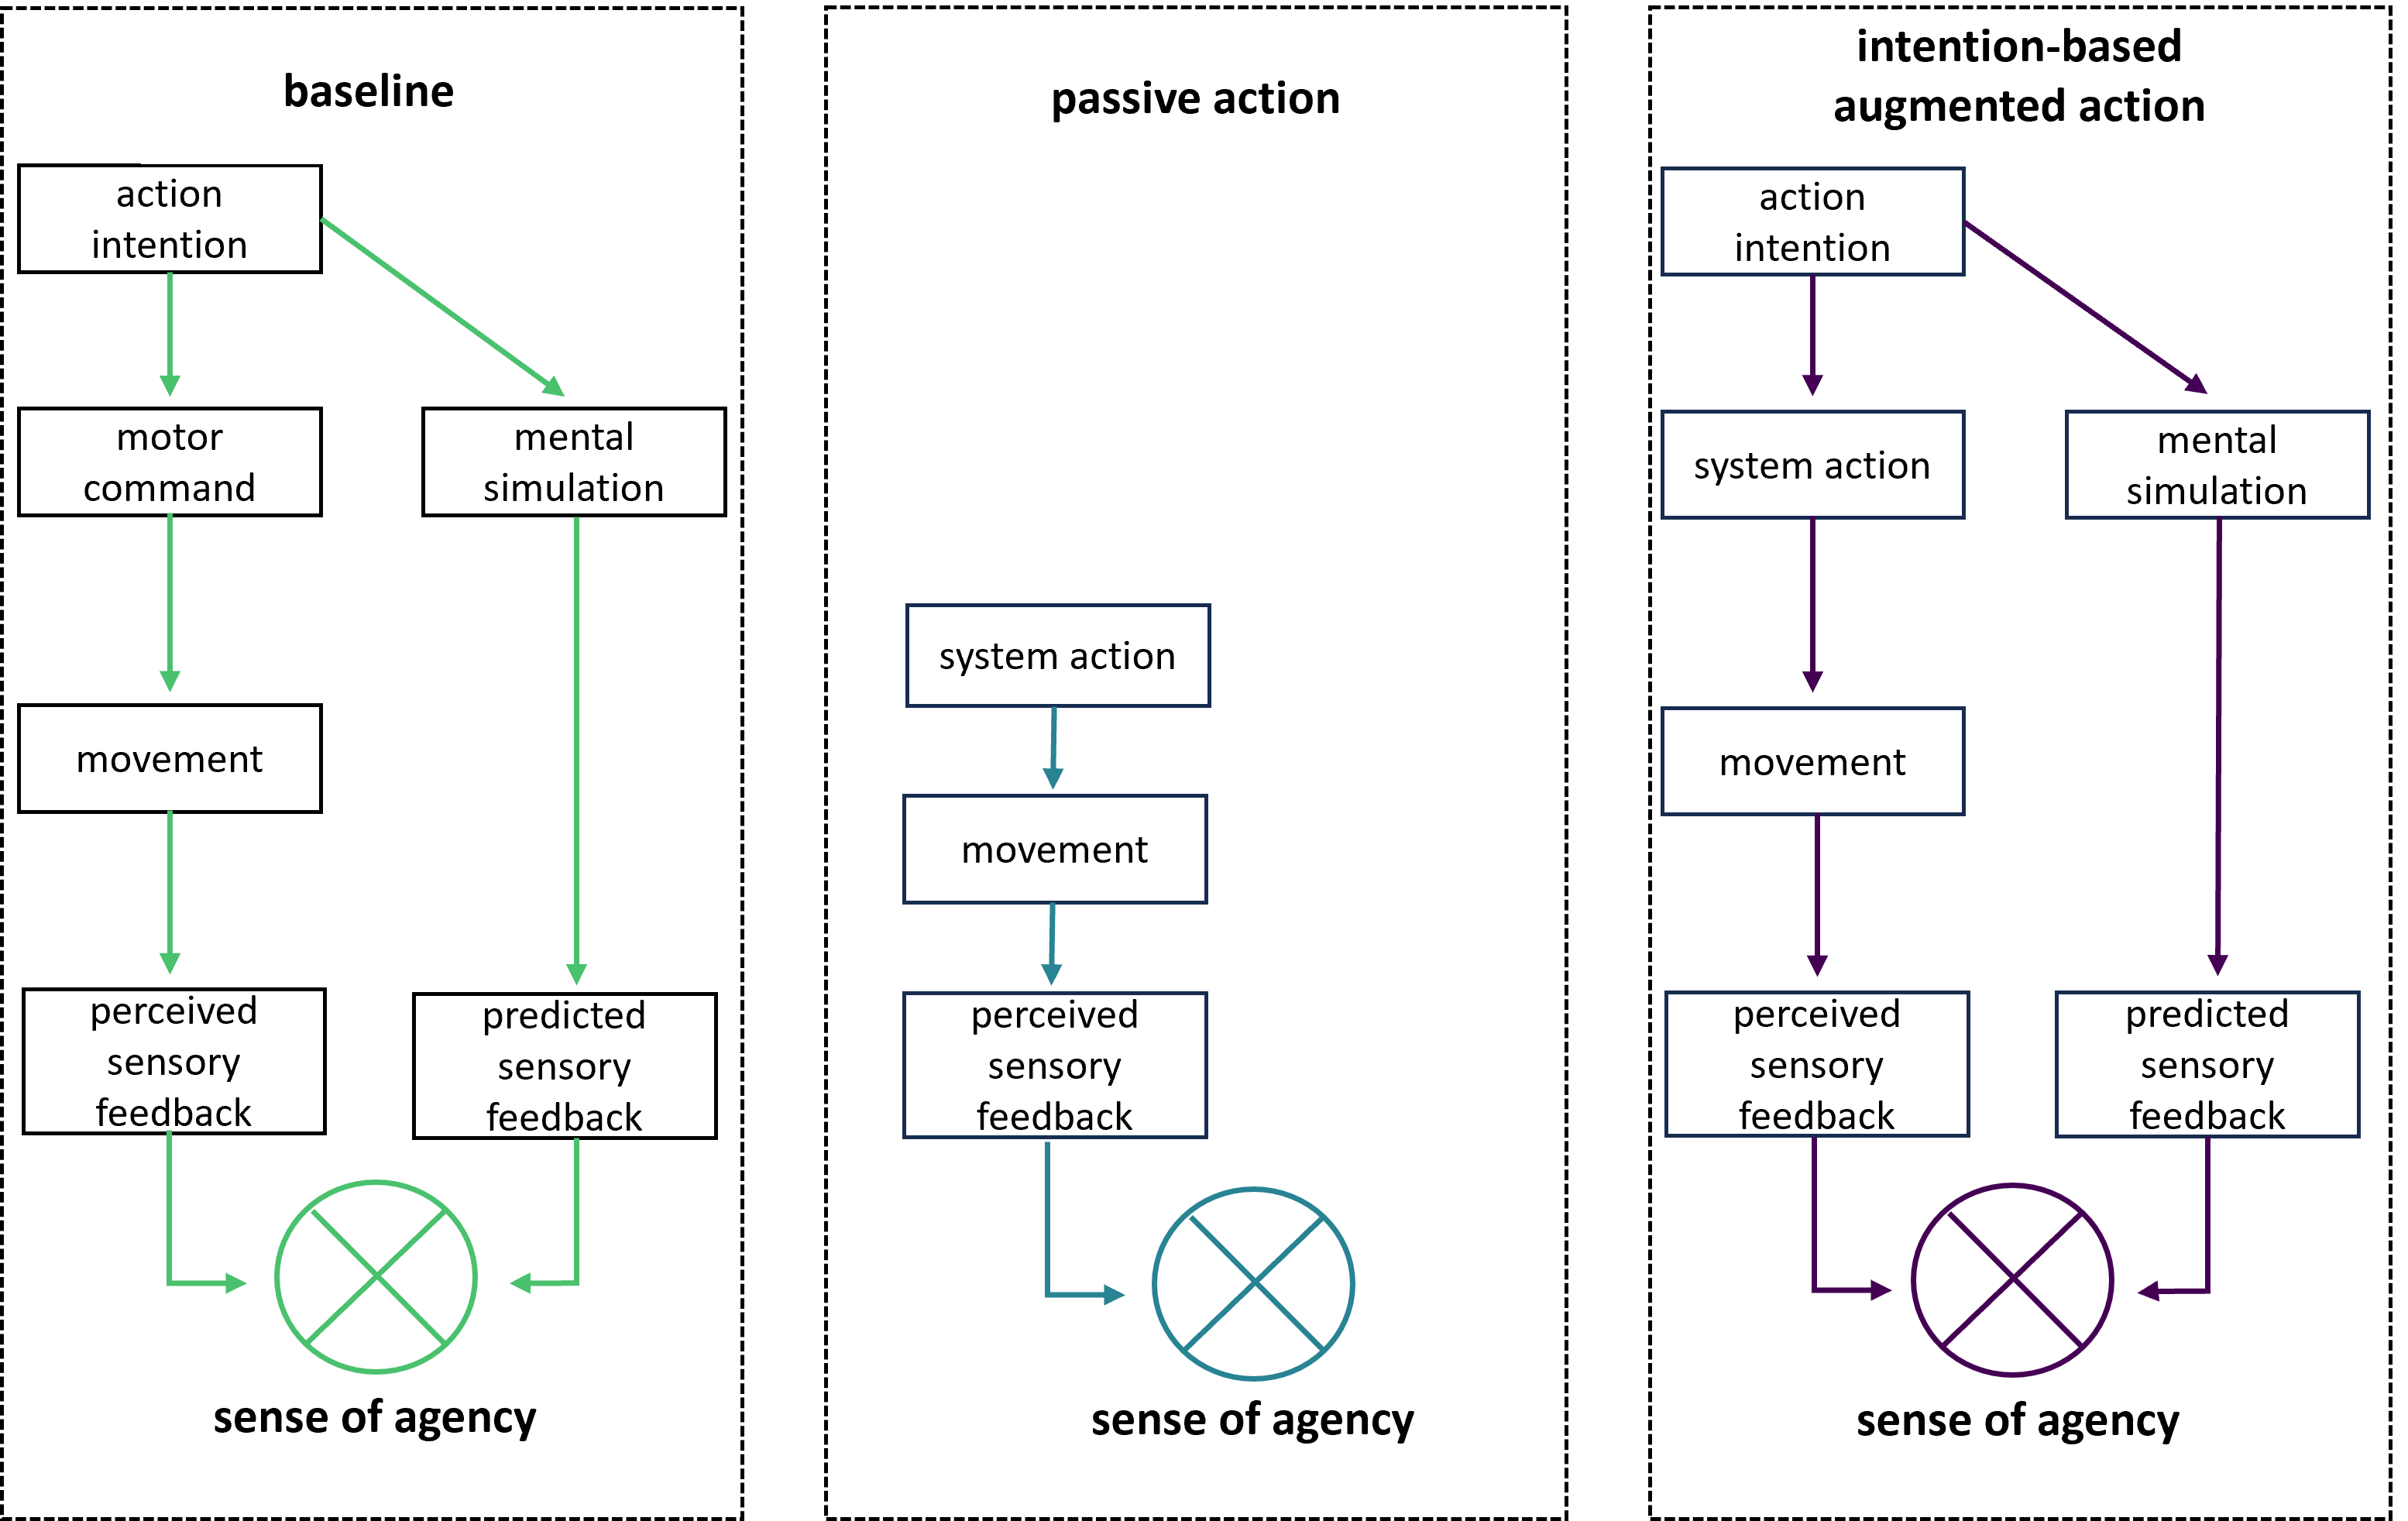
\includegraphics[width=\columnwidth]{figures/augmented_com_model_colour.png}
%     \caption{draft - visualization of comparator model of the SoA in the case of augmented interactions (inspired by Dewey 2019)}
%     \label{fig:com_model}
% \end{figure}

To control an interaction in real-time, the EEG-based RP classifier was used to discriminate between two user states: either the user was predicted to be in an \textit{idle} state, reflecting the absence of an intent to act-- or the user was predicted to be in a \textit{pre-movement} state, indicating the presence of an intent to act. When the system predicted a \textit{pre-movement} state, the user's action was augmented, potentially even before their own voluntary motor command. In our user study, we then applied a mixed-methods research approach to investigate whether keeping the physical impact on the user's body in line with their intention to move preserves their SoA.






%%% Resources
% add results and general outcomes here?

% for now moved to introduction section
% We follow classical work in the neuroscience describing SoA as a bias in the perception of action \textit{outcome}: Intentional binding paradigms state that when a button press is followed by a -- delayed -- outcome, participants mentally compress the delay and reproduce it as such. Critically, this temporal compression only occurs following endogenous movement intention. The action outcome is mentally \textit{binded} to the intention. To reduce uncertainty about the binding, the brain `explains away' the excess delta, compressing the action-outcome delay <REF>.

% We found ... rendering the augmentation a \textit{natural}, integrated expansion of the user's body.



% By controlling the stimulus presentation, the experimenter can control the timing of the \textit{pre-emptive} gain of the user's action augmentation. 

% Resources
% The authors found a relation between the experience of agency and the \textit{pre-emptive} gain, i.e., how much earlier the action of the user could be elicited. However, setting this gain factor only works in stimulus-response scenarios where the user behavior can be predicted with high accuracy. 

% At around 80 ms preceding the naturally occurring action, user's integrate the augmentation and maintain an experience of agency. 

% if something happens for you in an interaction there is a cost to that:
% - impacts SoA which in turn may makes user's engage less -> citation?
% - may impact precision and accuracy, which can be very critical in high stakes scenarios, e.g. air traffic control -> citation?